%!TEX root = ../main.tex
\setcounter{chapter}{-1}
\chapter*{Introduction.}
%
% \section*{Introduction}
	In this case study corresponding to the course \emph{Multivariable Control and Coordination Systems}, we aim at putting into practice the concepts and methods presented in the lectures, as well as at providing a quick glance at how Matlab-Simulink can be used to simulate dynamical systems, implement control strategies, and assess control results.
	\par
	%
	One exercise is proposed, which are inspired on the challenges that automated vehicles must address.
	Specifically, we will address a simplified version of the so-called path tracking problem. 
	The path tracking problem refers to the challenge of generating control inputs such that an automated vehicle tracks a reference path accurately.
	\par
	Due to the exceptional constraints we needs to handle during the this semester, we will carry out exercises related to simulation, control, and observation. 

	\paragraph{Files:}
	In every case-study session you will be provided with the description of the exercise, a Matlab script \texttt{exercise\#\_*.m} (which does not need to be modified), a Matlab class \texttt{utilities.m} (common to all exercises) gathering some auxiliary functions the exercise scripts will use, a Matlab-class named \texttt{ex\#.m} which includes the methods that you have to complete, and some Simulink files you also have to be completed.\par
	%
	% The fact that we are using a class to gather the functions you have to complete is simply for clarity proposes. 
	% The methods of such a class will then be called from the provided exercise script.\par
	%
	%Basic Matlab 
	%Although not too advanced Matlab skills are needed to complete the exercises, they will definitely come in handy to understand the provided code, and how the functions are integrated in the main script.\par
	%
	\paragraph{Evaluation}
	At the end of the course we expect you to submit a zip file (named \texttt{LastName}-\texttt{FirstName.zip}) with a total of 6 items:
	\begin{itemize}
		\setlength\itemsep{0em}
		%
		\item one pdf document report. 
		\item two \texttt{ex\#.m} files, one per session, containing the solution to the proposed exercises,
		\item and three Simulink files with the solution you implemented.
	\end{itemize}

	You are allowed to work in small groups (up to three people max) and we encourage you to discuss ideas to overcome the difficulties you might find.
	However keep in mind that the report \textbf{must} be written individually and we expect to find slightly different simulation results and discussions in each of them. 
	Note as well that assessing simulation results is crucial and a bad/good discussion can invalidate/validate good/bad results. 	
	\par
	%
	Important: Even though the Matlab and Simulink files are requested, \textbf{the evaluation of the solutions will be solely based on the pdf report}.
	Meaning that references in the pdf document to the Simulink files or Matlab code such as \emph{'as can be seen in the attached Simulink file'} or others of the sort will be ignored. 
	Do not expect us exploring the Matlab files to find the solutions.
	Everything you want us to take into account when grading the exercises must be included in the report. 
	The only purpose of requesting the Matlab files is guaranteeing the uniqueness of your solution.\par
	%
	Finally, note that this is the new adaptation of the case study we used in the past. 
	Thus, typos, bugs, and inconsistencies may be found throughout the handout and code.
	We kindly ask you to point out any flaw you find so that we can improve and update the material of this case study.
	%

	\paragraph{Starting point}
	Last but not least, you are expected to arrive to the first session of the case study with the solution of the modeling exercise proposed the 28th of September. 

\chapter{Modeling, linearization, and discretization}
\label{ch:modeling}
	Automated vehicles must follow paths that the vehicles' own decision-making layers generate to enable the vehicle to stay in its lane, change lanes, cross intersections, avoid collisions, etc. 
	Some path-tracking methods found in the literature tackle the challenge by exploiting a kinematic model of the vehicle that describes the vehicle's position w.r.t.\ to the path that is to be tracked.

	Consider a reference path defined by a function %
	$\pi : \mathbb{R}\to\mathbb{R}^3$, %
	that, given a distance %
	$s_\pi\in\mathbb{R}$ %
	along the path, outputs a tuple %
	$(x_\pi(s_\pi), y_\pi(s_\pi), \theta_\pi(s_\pi))$ %
	representing the x-y position %
	$(x_\pi(s_\pi), y_\pi(s_\pi))$, %
	and orientation %
	$\theta_\pi(s_\pi)$ %
	at %
	$s_\pi$. %
	Then, given a point %
	$P_r\in\mathbb{R}^2$ %
	positioned in the middle of the vehicle's rear bumper, and the point %
	$P_{r,\pi}\in\mathbb{R}^2$ %
	corresponding to the projection of %
	$P_r$ %
	in the path %
	$\pi$, %
	the position of a vehicle could be described by:
	\begin{itemize}
		\item the distance %
		$\pathCoor\in\mathbb{R}$ %
		along the path corresponding to the vehicle's projections, 
		\item the so-called \emph{lateral error} %
		$d\in\mathbb{R}$, %
		defined as %
		$d = ||P_r - P_{r,\pi}||$, %
		showing the distance to the path, and
		\item the so-called \emph{heading error} %
		$\theta_e \in \mathbb{R}$, %
		defined as %
		$\theta_e = (\theta - \theta_\pi)$, %
		showing the difference between the vehicle's yaw angle $\theta$ and the path's orientation %
		$\theta_\pi$ at $P_{r,\pi}$. 
		\end{itemize}
		The coordinates listed above are illustrated in Fig.\ \ref{fig:system}.

	\begin{figure}[!h]
		\centering
		\resizebox{ 300 px }{!}{
			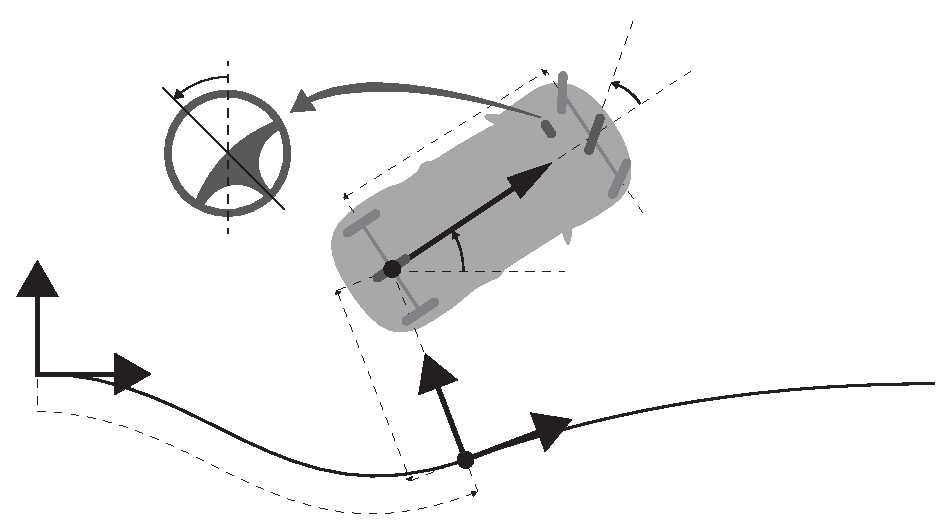
\includegraphics[width = 250px]{./_imags/system}
			\put(-187,0){$\pathCoor$}
			\put(-163,30){$\distToPath$}
			% \put(-55,110){$\yawErr$}
			\put(-85,120){$\frac{\steering}{16}$}
			\put(-205,121){$\steering$}
			\put(-127,70){$\yaw$}
			\put(-162,68){$P_r$}
			\put(-132,85){$\speed$}
			\put(-142,105){$\carLength$}
			\put(-128,05){$P_{r,\pi}$}
			\put(-28,38){$\pi$}
		}
		\caption{Coordinate system.}
		\label{fig:system}
	\end{figure}	
	%
	
	Representing by %
	$\phi\in\mathbb{R}$ %
	the position of the steering wheel (measured in radians), and assuming our control inputs to be the longitudinal speed reference %
	$v_{ref}\in\mathbb{R}^+$ %
	and the steering wheel's position reference %
	$\phi_{ref}\in[-4\pi, 4\pi]$, %
	the vehicle's model can be formulated as follows:
	\begin{subequations}
	\begin{align}	
		\dpathCoor 	& = \frac{\speed\cos(\yawErr)}{1-\distToPath\curvature} 
		\label{eq:non_linear_model_1}\\
		\ddistToPath& = \speed\sin(\yawErr) 
		\label{eq:non_linear_model_2}\\
		\dyawErr    & = \frac{\speed}{\carLength}\tan(\steering/16 ) - \curvature\dpathCoor 
		\label{eq:non_linear_model_3}\\
		\dspeed & = \accDyn(\speed_{ref}-\speed) 
		\label{eq:non_linear_model_4}\\
		\dsteering & = \steerDyn(\steering_{ref}-\steering) 
		\label{eq:non_linear_model_5}
	\end{align}
	\end{subequations}
	where %
	$\curvature$ %
	denotes the curvature of the path at %
	$\pathCoor$, %
	and %
	$\accDyn$ %
	and %
	$\steerDyn$ %
	represent the dynamic with which the speed and steering wheel references are followed.
	For the sake of further simplicity, from now on we will assume that the path has a constant curvature, i.e.\ %
	$\curvature = \kappa$. 
	\par
	%
	The states and control inputs of our system are
	\begin{align}
		\mathbf{\state} & = 
			\left[ \stat{1},\stat{2},\stat{3},\stat{4},\stat{5}\right] = %
			\left[\pathCoor, \distToPath, \yawErr, \speed, \steering\right] \label{eq:stateVector}, \\ 
		\mathbf{\control} & = 
			\left[ \con{1},\con{2} \right] = %
			\left[ \speed_{ref}, \steering_{ref} \right].
	\end{align}
	% which allows us writing the model in the form $ \mathbf{\dot{\state}} = f(\mathbf{\state},\mathbf{\control}) $ as
	% \begin{align}
	% 	%
	% 	%\dstat{1} 	& = \stat{7}\cos(\stat{3})\\
	% 	%\dstat{2} 	& = \stat{7}\sin(\stat{3})\\
	% 	%\dstat{3} 	& = \frac{\stat{7}}{L}\tan{\stat{8}}\\
	% 	%
	% 	\dstat{1} 	& = \frac{\stat{4}\cos(\stat{3})}{1-\stat{2}\curv} \label{eq:ss1}\\
	% 	\dstat{2}   & = \stat{4}\sin(\stat{3}) \label{eq:ss2}\\
	% 	\dstat{3}   & = \frac{\stat{4}}{\carLength}\tan(\stat{5}) - \frac{\curv\stat{4}\cos(\stat{3})}{1-\stat{2}\curv} \label{eq:ss3}\\
	% 	% \dstat{4}   & = \accDyn(\con{1}-\stat{4})\label{eq:ss4}\\
	% 	% \dstat{5}   & = \steerDyn(\con{2}-\stat{5}) \label{eq:ss5}
	% 	\dstat{4}   & = u_1\label{eq:ss4}\\
	% 	\dstat{5}   & = u_2 \label{eq:ss5}		
	% \end{align}
	% %
	% which is the system's continuous non-linear model we will use to design and implement the studied control and observation techniques. 
		
	Moreover, unless stated otherwise, we will consider the output of the system to be 
	\begin{align}
		\mathbf{y} = \mathbf{x}.
	\end{align}
	\section{Questions}
	Answer the following questions:
	\begin{itemize}
		\item Rewrite the non-linear model in the standard form $\mathbf{\dot{\state}} = f(\mathbf{\state},\mathbf{\control})$.
		\item Given the chosen state space, why it wouldn't be appropriate linearizing the system around a nominal \emph{point}.
		\item Calculate the \emph{nominal trajectory} representing the constant-speed perfect tracking situation (that is, a situation where the vehicle drives perfectly on the path and at a constant speed %
		$v_{ref}$) for a path of constant curvature $\curv_{ref}$. 
		\item Linearize the system around such a nominal trajectory.
		\item Discretize the system using Euler approximation. 
	\end{itemize}

